% Unofficial University of Cambridge Poster Template
% https://github.com/andiac/gemini-cam
% a fork of https://github.com/anishathalye/gemini
% also refer to https://github.com/k4rtik/uchicago-poster

\documentclass[final]{beamer}

% ====================
% Packages
% ====================

\usepackage[T1]{fontenc}
\usepackage{lmodern}
\usepackage[orientation=portrait,size=a0,scale=1.25]{beamerposter}
\usetheme{gemini}
\usecolortheme{nott}
\usepackage{graphicx}
\usepackage{booktabs}
\usepackage{tikz}
\usepackage{pgfplots}
\pgfplotsset{compat=1.14}
\usepackage{anyfontsize}


% for tables
\usepackage{multirow}
\usepackage{multicol}
\usepackage{transparent}

% for urls
\usepackage{hyperref}

% for subfigures
\usepackage{caption}
\usepackage{subcaption}

% for bibliography
\renewcommand{\refname}{Literature}
\usepackage[backend=biber]{biblatex}
\addbibresource{poster.bib}

% for inline code listings
\usepackage{listings}
\usepackage{xparse}
\usepackage{xcolor}
\definecolor{codeblue}{rgb}{0.0, 0.0, 1.0}
\definecolor{codegreen}{rgb}{0.0, 0.5, 0.0}
\definecolor{codegray}{rgb}{0.5, 0.5, 0.5}
\definecolor{codepurple}{rgb}{0.58, 0.0, 0.82}
\definecolor{backcolour}{rgb}{0.95, 0.95, 0.92}
\lstdefinestyle{py}{
  language=Python,
%   backgroundcolor=\color{backcolour},
  commentstyle=\color{codegreen},
  keywordstyle=\color{codeblue},
  numberstyle=\tiny\color{codegray},
  stringstyle=\color{codepurple},
  basicstyle=\small\ttfamily,
  breakatwhitespace=false,
  breaklines=true,
  captionpos=b,
  keepspaces=true,
  numbers=left,
  numbersep=5pt,
  showspaces=false,
  showstringspaces=false,
  showtabs=false,
  tabsize=4,
  frame=0,
  rulecolor=\color{black},
  morekeywords={self, assert, yield, None, True, False}
}

% ====================
% Lengths
% ====================

% If you have N columns, choose \sepwidth and \colwidth such that
% (N+1)*\sepwidth + N*\colwidth = \paperwidth
\newlength{\sepwidth}
\newlength{\colwidth}
\setlength{\sepwidth}{0.025\paperwidth}
\setlength{\colwidth}{0.45\paperwidth}

\newcommand{\separatorcolumn}{\begin{column}{\sepwidth}\end{column}}

% ====================
% Title
% ====================

% Title page
\title{\Large Network Diffusion --- Framework to Simulate Spreading Processes in Complex Networks}
\author{\large
    \textbf{Micha{\l} Czuba} \inst{1},
    Mateusz Nurek \inst{1},
    Damian Serwata \inst{1},
    Yu-Xuan Qi \inst{2},
    Mingshan Jia \inst{2},
    Katarzyna Musial \inst{2},
    Rados{\l}aw Michalski \inst{1},
    Piotr Br{\'o}dka \inst{1}
}
\institute[]{
  \inst{1} Wroc{\l}aw University of Science and Technology\\
  \inst{2} University of Technology Sydney
}

% ====================
% Footer (optional)
% ====================

\footercontent{
  \href{https://networks.pwr.edu.pl/}{https://networks.pwr.edu.pl} \hfill
  NetSci, Canada, July 2023 \hfill
  \href{mailto:michal.czuba@pwr.edu.pl}{michal.czuba@pwr.edu.pl}}

% ====================
% Logo (optional)
% ====================

\logoright{
\includegraphics[height=4cm]{logos/nsl-white.pdf}}
\logoleft{
\includegraphics[height=4cm]{logos/wust_logo.pdf}}

% ====================
% Body
% ====================

\begin{document}

\begin{frame}[t, fragile]
\begin{columns}[t]

\separatorcolumn
\begin{column}{\colwidth}

\begin{block}{Introduction}
    Spreading phenomena are one of the issues considered by a network science. They can be obeserved
    in various areas like: dynamics of political opinions, marketing campaigns, spread of epidemics,
    computer viruses, etc. With the advancement of computational network science analytical 
    approaches became insufficient for large graphs, prompting researchers to use computational
    methods. In recent years, the scope of network science has significantly expanded beyond static
    graphs to encompass more complex structures. The introduction of streaming, temporal, multilayer,
    and hypernetwork approaches has brought new possibilities and imposed additional requirements.
    Unfortunately, the pace of advancement is often too rapid for existing computational packages to
    keep up with the functionality updates...
\end{block}

\begin{alertblock}{Problem}
    There is a bunch of very good and robust tools that helps in sumulating diffusion processes in 
    networks, e.g. \lstinline[style=py]{ndlib} (which we love). \\
    \vspace{2em}
    However, if we consider...\\
    \vspace{1em}
    \hspace{5em}...more complex network models,... \\
    \vspace{1em}
    \hspace{5em}...spreading multiple processes at the same time... \\
    \vspace{1em}
    \hspace{14em}...\textbf{a gap among the available toolkits} emerges.
\end{alertblock}

\begin{block}{Our Contribution}
    In order to address the issue, we decided to redesign, polish, and share our internal 
    environment which we are using in the lab. Thus, we present
    \lstinline[style=py]{network-diffusion}. To start using library just type in your shell:
    \begin{center}
        \large
        \begin{verbatim}
            pip install network-diffusion
        \end{verbatim}
    \end{center}
    \vspace{-1em}
    Or scan this code to reach the docs with more examples:
    \begin{figure}
        
\includegraphics[width=15cm]{../presentation/figures/qr_code.pdf}
    \end{figure}
\end{block}

\begin{block}{Key Features}
    \begin{itemize}
        \item \textbf{End-to-End Simulation Workflow}: The library enables users 
        to simulate diffusion processes in complex networks with ease. Whether
        you are studying information spread, disease propagation, or any other
        diffusion phenomena, this library has you covered.
        \item \textbf{Support for Temporal Network Models}: You can work with temporal models, allowing you to
        capture the dynamics of processes over time. These temporal models can be
        created using regular time windows or leverage \textbf{CogSnet}.
        \item \textbf{Support for Multilayer Network Models}: The library supports multilayer networks, which are
        essential for modelling real-world systems with interconnected layers of
        complexity
        \item \textbf{Predefined Spreading Models}: You have the option to use predefined diffusion 
        models such as the Linear Threshold Model, Independent Cascade Model, and more. Those are
        implemented to simplify the simulation process, allowing users to focus on their specific
        research questions.
        \item \textbf{An Interface for Implementing Custom Spreading Models}: Additionally, 
        \lstinline[style=py]{network-diffusion} allows you to define your own diffusion models using
        open interfaces, providing flexibility for researchers to tailor simulations to their unique
        requirements.
        \item \textbf{New Centrality Measures}: The library provides a wide range of centrality 
        measures specifically designed for multilayer networks. These measures can be valuable for
        selecting influential seed nodes in diffusion processes.
        \item \textbf{NetworkX Compatibility}: The package is built on top of  
        \lstinline[style=py]{networkx}, ensuring seamless compatibility with this popular Python 
        library for network analysis. You can easily integrate it into your existing
        \lstinline[style=py]{networkx}-based workflows.
    \end{itemize}
\end{block}

\end{column}

\separatorcolumn
\begin{column}{\colwidth}

\begin{alertblock}{Extending the LTM to multilayer networks}
    Linear Threshold Model in its initial form~\cite{kempe2003maximizing} cannot be directly applied to multilayer networks --- \textbf{actors are the subject of the process, while the nodes are their auxiliary representation}...
    Therefore, we need to define:
    \begin{itemize}
        \item what does it mean that an actor is (or is not) active,
        \item how does it relate to diffusion dynamics taking place within 
        layers, where it is represented.
    \end{itemize}
    In our research, we used the approach proposed by~\cite{zhong2022mltm} with amendments so that a homogeneity among actors has been imposed in the sense of an activation threshold ($\mu$) and a protocol (v.i.).

    \heading{Protocol function in MLTM}\label{def:proto}
        According to~\cite{zhong2022mltm}, state of the actor $n$ of a multilayer network $M = (N, L, V, E)$ in the time step $t$ is determined
        by a following function: 
        \begin{equation*}
            x_{n}(t) =
            \begin{cases}
              1,  & \text{if \space} y_{n}(t) \geq \delta \text{\space or 
                \space} x_{n}(t-1) = 1 \\
              0,  & \text{otherwise}
            \end{cases} 
        \end{equation*}
        Where:
        \begin{description}
            \item[$\delta$] - a parameter of the model, $\delta \in [\frac{1}{|L|}, 1]$,
            \item[$y_{n}(t)$] - a mean input of actor $n$ (represented in $K$ layers) in time $t$, $y_{n}(t) = |K|^{-1} \sum_{k \in K} y_{v}^{k}(t)$.
            \item[$y_{v}^{k}(t)$] - an impulse of node $v$ from layer $k$ in time $t$, $y_{v}^{k}(t) \in \{0, 1\}$
        \end{description}

    \heading{Toy example}
    \textbf{We decided to examine two extreme cases: $\mathbf{\delta = 1}$ ($\mathbf{AND}$) and $\mathbf{delta = \frac{1}{L}}$ ($\mathbf{OR}$)}. In the former one, an actor gets activated if it receives sufficient influence on all layers where it is represented, and conversely the latter, where sufficient input in at least one layer is enough for activation.
    \begin{figure}
        \centering
        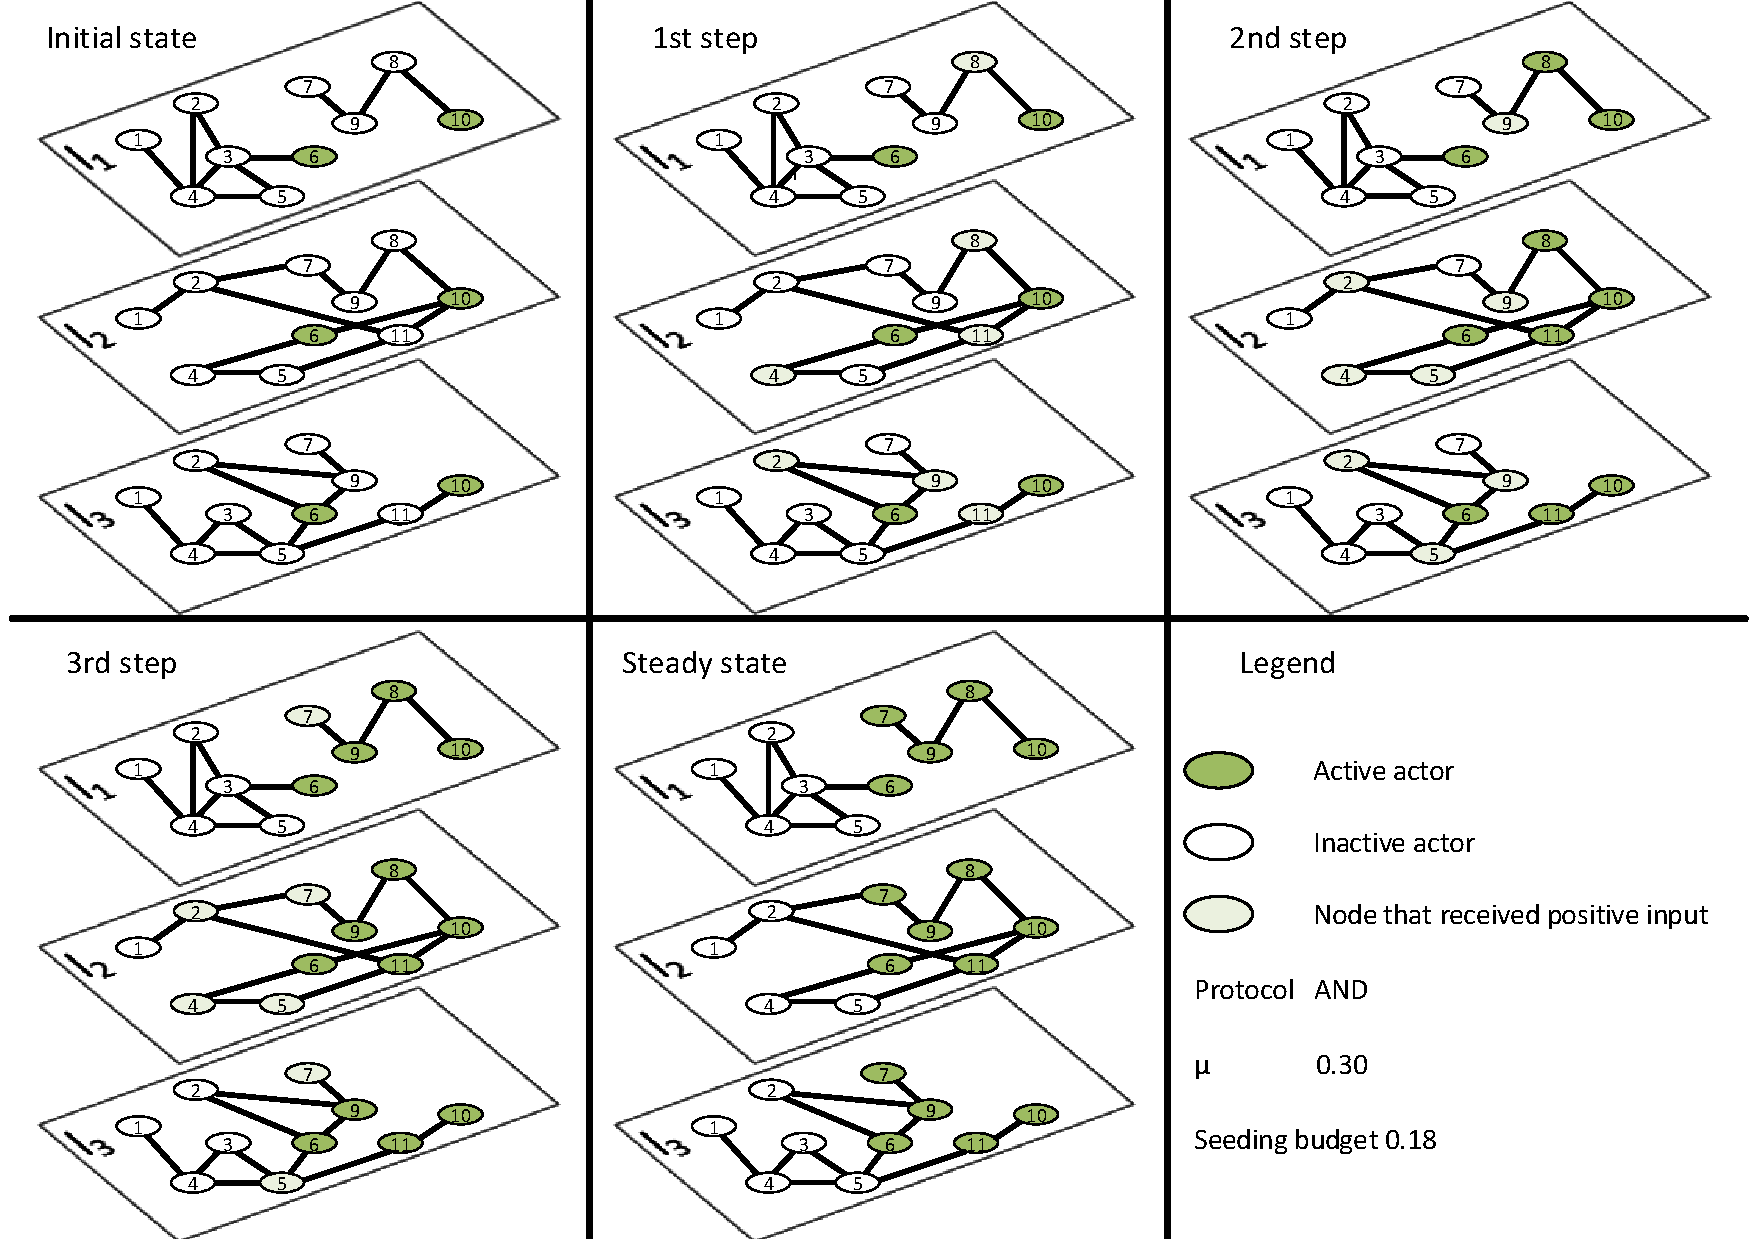
\includegraphics[width=1\linewidth]{figures/ltm_example.pdf}
        \caption{Example of spreading of MLTM in toy network with protocol $AND$.}
        \label{fig:ltm_example_and}
    \end{figure}
\end{alertblock}

\begin{block}{A problem we tackled}
    \heading{Budget constrained influence maximisation}
    Let $\mathcal{S}$ be a family of sets of cardinality $s$ over actors of
    the multilayer network $M$ in the sense that $\mathcal{S} \subseteq
    powerset(N)$. Let $\sigma: \mathcal{S} \rightarrow \mathbb{R^{+}}$ b
    an arbitrary function that maps a set of actors used as a seed set to
    a number denoting the expected size of activated actors in a binary discrete system. An influence maximisation problem for seeding budget of size $s$ is an issue of finding $ S_{0}: \arg\max(\sigma) = S_{0} \wedge |S_{0}| \leq s$.
    
    \heading{Measuring an efficiency of the diffusion}
    We used \textbf{Gain} metric to assess a performance of the spreading model that bases on a number of seeds, a number of actors that could be activated, and a number of active actors when diffusion faded down:
    \begin{equation*}
        G = 100 \cdot \frac{|S_{D} - S_{0}|}{|N - S_{0}|}
    \end{equation*}
\end{block}

\begin{block}{Seed selection methods}
    During the study, we evaluated the following methods to select seed set for MLTM:
    \begin{itemize}
        \item degree (\textit{deg-c)},
        \item neighbourhood size (\textit{nghb-1s}, \textit{nghb-2s}),
        \item PageRank (\textit{p-rnk}, \textit{p-rnk-m}),
        \item VoteRank (\textit{v-rnk}, \textit{v-rnk-m}),
        \item k-shell decomposition (\textit{k-sh}, \textit{k-sh-m}),
        \item random choice (\textit{random}),
        \item greedy (\textit{greedy}).
    \end{itemize}
    We used two ideas to adapt PageRank, VoteRank, and k-shell to multilayer networks: compute the metric for each layer and take its mean value for each actor (e.g. \textit{p-rnk}) or replace Degree Centrality with Neighbourhood Size in the algorithm (e.g. \textit{p-rnk-m}).
\end{block}



% \begin{block}{Used data and parameter space}
%     \begin{table}
%     \begin{subtable}[t]{0.45\textwidth}
%         \caption{}
%         \resizebox{\columnwidth}{!}{%
%             \begin{tabular}{lllllp{14cm}}
%                 \hline Name & Layers & Actors & Nodes & Edges & Note \\ \hline
%                 aucs & 5 & 61 & 224 & 620 & AUCS CS-AARHUS \\
%                 ckmp & 3 & 241 & 674 & 1370 & Coleman, Katz, Menzel Innovation Among Physicians \\
%                 eutr-A & 37 & 417 & 2034 & 3588 & The European Air Transport Network \\
%                 lazega & 3 & 71 & 212 & 1659 & Lazega Law Firm \\ \hline
%                 er-2 & 2 & 1000 & 2000 & 5459 & \multirow{3}{*}{\parbox{14cm}{Erdős–Rényi networks generated with multinet library}} \\
%                 er-3 & 3 & 1000 & 3000 & 7136 & \\
%                 er-5 & 5 & 1000 & 5000 & 15109 & \\ \hline
%                 sf-2 & 2 & 1000 & 2000 & 4223 & \multirow{3}{*}{\parbox{14cm}{Scale-free networks generated with multinet library}} \\
%                 sf-3 & 3 & 1000 & 3000 & 5010 & \\
%                 sf-5 & 5 & 1000 & 5000 & 10181 & \\ \hline
%             \end{tabular}%
%         }
%         \label{tab:networks_eda}
%     \end{subtable}
%     \hspace{\fill}
%     \begin{subtable}[t]{0.45\textwidth}
%         \caption{}
%         \resizebox{\columnwidth}{!}{%
%         \begin{tabular}{lp{10cm}p{10cm}}
%             Protocol & $OR$ & $AND$ \\ \hline
%             $s$ range & $[1, 2, ..., 10, 15, 20, 25, 30]$ & $[15, 20, 25, 30, 31, ..., 40]$ \\ \hline
%             $\mu$ range & \multicolumn{2}{p{20cm}}{$[0.1, 0.2, 0.3, 0.4, 0.5, 0.6, 0.7, 0.8, 0.9]$} \\ \hline
%             networks & \multicolumn{2}{p{20cm}}{real (aucs, ckmp, lazega, eutr-A), Erdős–Rényi (er-2, er-3, er-5), Scale-free (sf-2, sf-3, sf-5)} \\ \hline
%             s.~s.~method & \multicolumn{2}{p{20cm}}{deg-c, greedy, k-sh, k-sh-m, nghb-1s, nghb-2s, p-rnk, p-rnk-m, random, v-rnk, v-rnk-m} \\
%         \end{tabular}%
%         }
%         \label{tab:parameter_space}
%     \end{subtable}
%     \caption{Networks used in experiments with their basic parameters shortlisted (tab.~\ref{tab:networks_eda}), values of each evaluated parameter - in total 27,720 executed experiments (tab.~\ref{tab:parameter_space}).}
%     \end{table}
% \end{block}



\begin{alertblock}{A Short Example}
\begin{lstlisting}[style=py, basicstyle=\footnotesize\ttfamily]
import network_diffusion as nd

# define the model with its internal parameters
spreading_model = nd.models.MICModel(
    seeding_budget=[90, 10, 0],  # 95% act suspected, 10% infected, 0% recovered
    seed_selector=nd.seeding.RandomSeedSelector(),  # pick infected act randomly
    protocol="OR",  # how to aggregate impulses from the network's layers
    probability=0.5,  # probability of infection
)

# get the graph - a medium for spreading
network = nd.mln.functions.get_toy_network_piotr()

# perform the simulation that lasts four epochs
simulator = nd.Simulator(model=spreading_model, network=network)
logs = simulator.perform_propagation(n_epochs=3)

# obtain detailed logs for each actor in the form of JSON
raw_logs_json = logs.get_detailed_logs()

# or obtain aggregated logs for each of the network's layer
aggregated_logs_json = logs.get_aggragated_logs()

# or just save a summary of the experiment with all the experiment's details
logs.report(visualisation=True, path="my_experiment")
\end{lstlisting}
\end{alertblock}
    
% \begin{exampleblock}{Try the Library}
%     To start using library just type in your shell:
%     \begin{center}
%         \large
%         \begin{verbatim}
%             pip install network-diffusion
%         \end{verbatim}
%     \end{center}
%     \vspace{-1em}
%     Or scan this code to reach the docs with more examples:
%     \begin{figure}
%         
\includegraphics[width=10cm]{../presentation/figures/qr_code.pdf}
%     \end{figure}
% \end{exampleblock}

\begin{block}{References}
    \printbibliography
\end{block}

\end{column}
\separatorcolumn

\end{columns}
\end{frame}

\end{document}
